\chapter{Review of Related Literature}\label{cha: literature-review}
\section{Terahertz photoconductive antenna}\label{sec: thz-pca}
The range of frequencies between microwave and infrared in the electromagnetic spectrum is known as the \gls{THz} range. It was also called the \gls{THz} gap in the past due to the difficulty of finding emitters and detectors which worked in this frequency range\cite{alfihedDevelopmentsIntegrationApplication2020}.\ \gls{THz} radiation is non-ionizing and can penetrate through organic material such as plastic and clothing, thus it has potential use in biological characterization\cite{yuMedicalApplicationTerahertz2019}, detection of contraband materials\cite{kawaseNondestructiveTerahertzImaging2003}, and chemical identification\cite{zhongIdentificationClassificationChemicals2006}. Some substances have specific \gls{THz} absorption spectra which can be used to identify their composition, as shown in~\ref{fig: thz_substance}. The interaction amongst the bonds and forces in the molecules result in vibrational modes visible in the THz region\cite{kawaseNondestructiveTerahertzImaging2003}. On the other hand, THz reflection can be used to detect concealed objects when the concealing material is transparent to THz radiation as in ref{through}, as the case for dielectrics such as clothing\cite{chengEnhancingConcealedObject2025}. A common setup for some of these applications involves \gls{THz} \gls{TDS}.

\begin{figure}
	\centering
	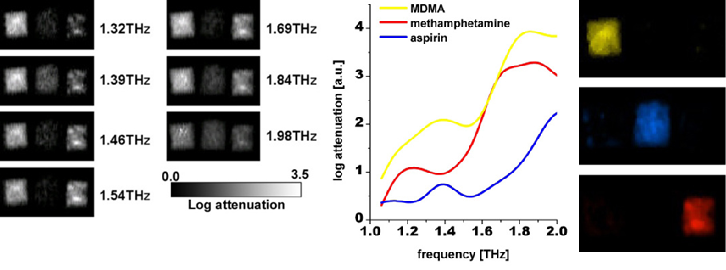
\includegraphics[width=0.85\textwidth]{figures/thz_subs.png}
	\caption[THz spectra of substances]{THz identification of MDMA, methamphetamine, and aspirin through a paper envelope. The substances are differentiated using their THz spectra\cite{kawaseNondestructiveTerahertzImaging2003}}\label{fig: thz_substance}
\end{figure}
In \gls{THz} \gls{TDS}, a \gls{THz} pulse is generated using a \gls{PCA}. The shape of the electrodes influences the pattern of the \gls{THz} radiation generated by the \gls{PCA}. Dipole and bowtie patterns demonstrate higher polarization ratios compared to spiral antennas while spiral and log-spiral antennas have a higher calculated radiation efficiency compared to bowtie and dipole antennas\cite{gonzalezComparisonDipoleBowtie2005}. The shapes of the antennas are presented in~\ref{fig: antenna}.

\begin{figure}
	\centering
	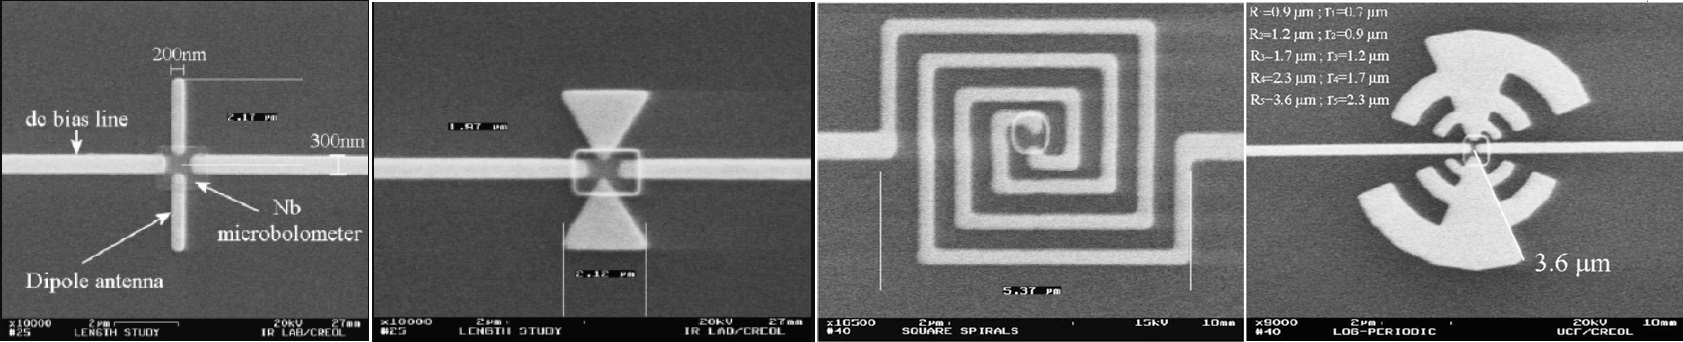
\includegraphics[width=0.95\textwidth]{figures/antenna.jpg}
	\caption[PCA geometries]{Commonly used THz PCA geometries; from left to right: dipole, bowtie, spiral, and log-spiral\cite{gonzalezComparisonDipoleBowtie2005}}\label{fig: antenna}
\end{figure}
The emission mechanism for the \gls{PCA} is as follows: the photoconductive material between the electrodes is illuminated with a femtosecond laser pulse, which generates photocarriers that are swept by an electric field applied to the electrodes of the \gls{PCA}\cite{burfordReviewTerahertzPhotoconductive2017, songHandbookTerahertzTechnologies2015}. The transient current $i_{PC}\left ( t \right )$ resulting from the moving carriers generates electromagnetic radiation according to Maxwell's equations, with the intensity of the electric field component of the THz wave radiated by a dipole antenna expressed by\ref{eqn:THz_electric}
\begin{equation}\label{eqn:THz_electric}
	E_{THz}\left ( \textit{r},\theta ,\textit{t} \right )= \frac{l_{e}}{4 \pi \varepsilon c^{2} r}\frac{\partial i_{PC}\left ( t \right )}{\partial t}\sin\left ( \theta  \right )
\end{equation}
where $l_{e}$ is the antenna length, $\varepsilon$ the permittivity, $c$ the speed of light, $r$ the distance from the dipole, and $\theta$ the angle relative to the dipole axis\cite{songHandbookTerahertzTechnologies2015}. 

The transient current density term $i_{PC}\left ( t \right )$  is proportional to the convolution integral of the carrier density $n\left ( t \right )$ and electron velocity $v_{e}\left ( t \right )$ as shown in~\ref{eqn:transient}\cite{songHandbookTerahertzTechnologies2015}.
\begin{equation}\label{eqn:transient}
	i_{PC}\left ( t \right )\propto P_{pulse}\left ( t \right )\otimes \left ( n\left ( t \right )v_{e}\left ( t \right ) \right ).
\end{equation}

The carrier density is described by
\begin{equation}\label{eqn:density}
	\frac{dn}{dt} = \eta \frac{P_{\text{pulse}}(t)}{h\nu} - \frac{n}{\tau_c}
\end{equation}

and using a $1$D Drude-Lorentz model, the electron velocity by 
\begin{equation}\label{eqn:e_velocity}
	\frac{dv_e}{dt} = -\frac{v_e}{\tau_s} + \frac{e}{m^*} E
\end{equation}

where $\eta$ is the absorption efficiency, $P_{\text{pulse}}(t)$ the ultrashort laser pulse power considered over time,  $\tau_c$, $\tau_c$, and $m^*$ the carrier lifetime, momentum relaxation time, electron effective mass respectively, and $E$ the local electric field\cite{songHandbookTerahertzTechnologies2015}.

A photoconductive antenna is also used to detect THz radiation, with the incoming THz pulse focused together with a femtosecond pulse split from the same source at the gap of the antenna. As the femtosecond probe pulse arrives at the gap, carriers are excited and then accelerated proportionally by the electric field provided by the incoming THz pulse\cite{burfordReviewTerahertzPhotoconductive2017}. The difference of the probe pulse and the THz pulse provides a measurement in the time domain for the transient of the THz pulse. A schematic of a complete THz TDS system with emitter and detector is shown in~\ref{fig: thz_tds}. Some of the photoconductive materials used for THz TDS systems include \gls{LT} grown GaAs and InGaAs\cite{gregoryHighResistivityAnnealed2003, metzgerStructuralElectricalProperties1993, mellochLowTemperatureGrownIIIV1995}. LT-GaAs is grown via molecular beam epitaxy at $\qtyrange{200}{300}{\degreeCelsius}$ instead of the usual growth temperature around $\qty{600}{\degreeCelsius}$\cite{mahalingamSubstrateTemperatureDependence1991}..

\begin{figure}
	\centering
	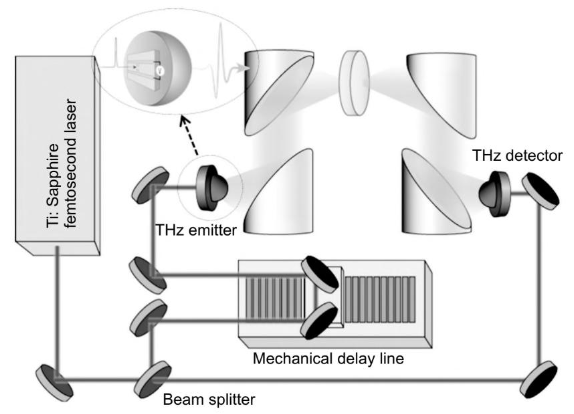
\includegraphics[width=0.8\textwidth]{figures/thz_tds.png}
	\caption[THz TDS setup]{Schematic of a THz TDS setup with a femtosecond laser and two photoconductive antennas\cite{songHandbookTerahertzTechnologies2015}}\label{fig: thz_tds}
\end{figure}

\section{Electromagnetic Waves in Dielectric Materials}\label{sec: EM waves}
The propagation of electromagnetic waves through dielectric materials can be described using the Fresnel equations, which can be derived from the boundary conditions that constrain the electric and magnetic field components arising as a direct result of Max\-well's equations. 
Suppose incident light approaches a boundary between two dielectric materials with refractive indices $n_1$ and $n_2$ as shown in~\ref{fig: polarization}. The first case shows s-polarized light, where the electric field is perpendicular to the plane of incidence, while the second case shows p-polarized light, where the electric field is parallel to the plane of incidence. The incident and reflected angles are equal $\theta_i = \theta_r$, and the transmitted angle is given by Snell's law $n_1\sin \theta_i = n_2 \sin \theta_t$. The boundary conditions require that the components of the electric and magnetic fields be continuous, thus for s-polarized light, the electric fields are given by $E_i + E_r = E_t$ or $1 + r = t$, where $r$ and $t$ are the reflected and transmitted amplitudes and the incident amplitude is normalized to $1$. The y-component of the magnetic field is given by $H_i \cos \theta_i - H_r \cos \theta_r = H_t \cos \theta_t$, which can be rewritten as $n_1 \cos \theta_i (1 - r) = n_2 \cos \theta_t t$ using the relation $H = n E / c$. Solving for $r$ gives 
\begin{equation} \label{eqn: reflection_s-polarized}
		r_s = \frac{n_1 \cos \theta_i - n_2 \cos \theta_t}{n_1 \cos \theta_i + n_2 \cos \theta_t}
\end{equation}
while solving for $t$ gives
\begin{equation} \label{eqn: transmission_s-polarized}
		t_s = \frac{2 n_1 \cos \theta_i}{n_1 \cos \theta_i + n_2 \cos \theta_t}.
\end{equation}
For p-polarized light, the magnetic fields are given by $H_i + H_r = H_t$ or $n_1 (1 + r) = n_2 t$, thus the electric fields are given by $E_i \cos \theta_i - E_r \cos \theta_r = E_t \cos \theta_t$, which can be rewritten as $n_1 (1 - r) \cos \theta_i = n_2 t \cos \theta_t$. Solving for $r$ gives
\begin{equation} \label{eqn: reflection_p-polarized}
		r_p = \frac{n_2 \cos \theta_i - n_1 \cos \theta_t}{n_2 \cos \theta_i + n_1 \cos \theta_t}
\end{equation}
while solving for $t$ gives
\begin{equation} \label{eqn: transmission_p-polarized}
		t_p = \frac{2 n_1 \cos \theta_i}{n_2 \cos \theta_i + n_1 \cos \theta_t}.
\end{equation}

\begin{figure}
	\centering
	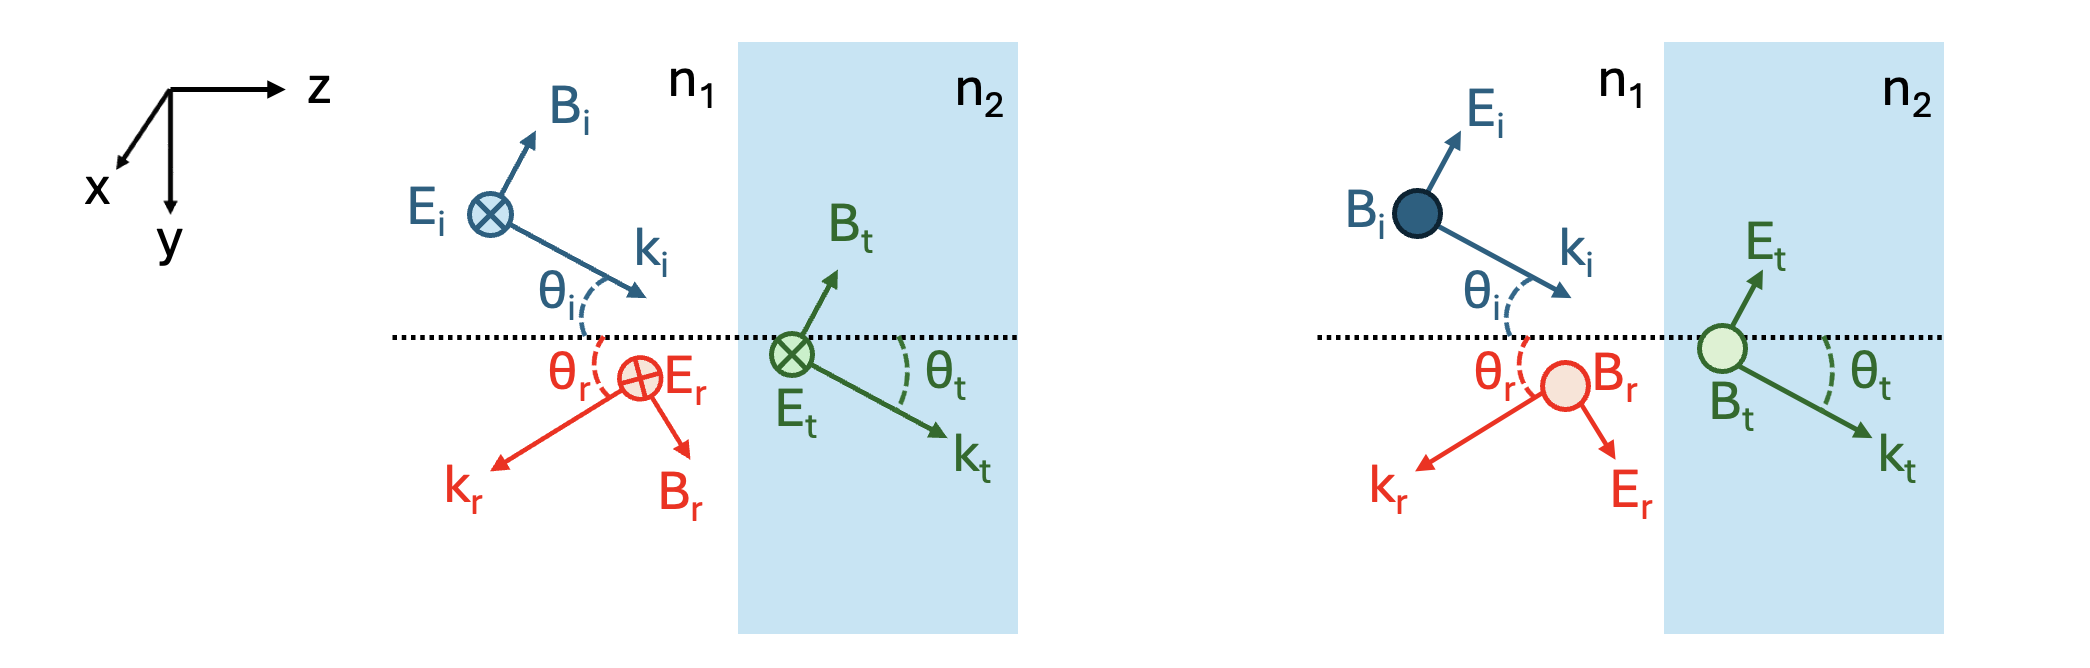
\includegraphics[width=0.85\textwidth]{figures/polarization.png}
	\caption[Polarization at two interfaces]{Diagram of polarized light at two interfaces. The left image shows the case for s-polarized light, with the electric field pointing into the page. For p-polarized light on the right the magnetic field points outside of the page.}\label{fig: polarization}
\end{figure}

At normal incidence the reflectance $R$ evaluates to 
\begin{equation} \label{eqn: reflectance_sqd}
		R=r_12^2={\left| {\frac{n_1-n_2}{n_1+n_2}} \right|}^2.
\end{equation}
For an uncoated glass substrate ($n_{\text{glass}} \approx 1.5$) in air ($n_{\text{air}} \approx 1.0$), approximately $4\%$ of incident light power is reflected per interface (Keshavarz Hedayati Elbahri, 2016; Raut et al., 2011). For high-index semiconductor materials like silicon or GaAs ($n_{\text{Si}} \approx 3.7$ at \qty{780}{\nano\meter}), reflection losses exceed $30\%$ (Keshavarz Hedayati Elbahri, 2016).

Consider a single dielectric film of thickness $d_2$ and refractive index $n_2$ deposited between an ambient medium $n_1$ (air) and a substrate $n_3$, where $n_1 < n_2 < n_3$ as shown in~\ref{fig: propagation}. The reflectance of the structure at normal incidence would be given by
\begin{equation} \label{eqn: reflectance_film}
		R=\frac{r^2_{12}+r^2_{23}+2r_{12}r_{23}\cos(2\delta_2)}{1+r^2_{12}+r^2_{23}+2r_{12}r_{23}\cos(2\delta_2)}
\end{equation}
where $\delta_2=k_2d_2={2\pi n_2 d_2}/{\lambda}$ is the phase difference between the reflected light at the interfaces of the dielectric film. The $2r_{12}r_{23}\cos(2\delta_2)$ term oscillates, and at $\cos(2\delta_2)=\pm 1$ or when $2\delta_2$ is an integer multiple of $2\pi$, interference of the reflected waves occur and the reflectance is at an extremum. The wavelength at the extremum is 
\begin{equation} \label{eqn: extremum}
		\lambda=\frac{2n_2d_2}{m}
\end{equation}
where $m$ is the number of cycles from one extremum to another. The refractive index of the thin film can be calculated if the thickness is known
\begin{equation} \label{eqn: index_extrema}
		n_2=\frac{m\lambda_1\lambda_m}{2d_2(\lambda_m-\lambda_1)}.
\end{equation}
and the new $\lambda$ is the average of the two wavelengths $\lambda=(\lambda_m+\lambda_1)/2$.

The mechanism of classical thin-film \gls{ARC}s relies on destructive wave interference (Raut et al., 2011).  Two necessary conditions must be satisfied simultaneously to achieve zero reflectance ($R = 0$) at a specific target wavelength $\lambda_t$. The first condition is that the optical path difference between the partial wave reflected from the top interface ($r_1$) and the partial wave reflected from the substrate interface ($r_2$) must result in a $\pi$ phase shift ($180^\circ$ out of phase). The physical film thickness $d$ must satisfy:
\begin{equation} \label{eqn: film_thickness}
		d = \frac{\lambda_t}{4 n_2}.
\end{equation}

Since both reflection events occur at interfaces transitioning from a lower to a higher refractive index ($n_1 < n_2$ and $n_2 < n_3$), both undergo an phase change upon reflection. The round-trip optical path within the coating $2 n_2 d_2 = {\lambda_t}/{2}$ introduces a net phase change of $\pi$, ensuring destructive interference.

The second condition for zero reflectance is that the intensities of the two reflected waves must be identical $\vert{}r_1\vert{} = \vert{}r_2\vert{}$. Equalizing the Fresnel reflection coefficients yields:
\begin{equation} \label{eqn: index_single}
		\frac{n_2 - n_1}{n_2 + n_1} = \frac{n_3 - n_2}{n_3 + n_2} \implies n_2 = \sqrt{n_1 n_3}.
\end{equation}

For a glass substrate ($n_3 = 1.5$) in air ($n_1 = 1.0$), the ideal coating index is $n_2 \approx 1.22$ (Keshavarz Hedayati Elbahri, 2016). However, finding natural bulk dielectric materials with $n \approx 1.22$ is difficult; magnesium fluoride ($\text{MgF}_2$, $n \approx 1.38$) is usually employed as an alternative (Keshavarz Hedayati Elbahri, 2016). Single-layer \gls{ARC}s suffer from multiple limitations. First, destructive interference is exact only at the design wavelength $\lambda_0$. At adjacent wavelengths the reflection increases rapidly. Another limitation of single-layer \gls{ARC}s is that off-normal angles of incidence alter both the internal propagation path length and the polarization-dependent reflection coefficients, shifting the minimum reflection dip away from $\lambda_t$.

To achieve broadband and wide-angle antireflection, multi-layer dielectric stacks comprising alternating high-index and low-index thin films are used (Astrauskytė et al., 2023). Multi-layer structures introduce multiple internal reflection pathways that result in broader and more easily tailored destructive interference minima across the relevant spectrum. The design of multi-layer \gls{ARC}s is usually performed computationally with the transfer matrix method\cite{sharhanTransferMatrixMathematical2020}.

\section{Transfer Matrix Method}\label{sec: TMM}
At the boundary between two dielectric materials, the electric field amplitudes of the incident, reflected, and transmitted waves can be related using a transfer matrix. In the schematic shown in~\ref{fig: propagation}a, a wave with amplitude $E_1^+$ is moving to the right, and another wave with amplitude $E_1^-$ is moving to the left. For the other side of the boundary, the amplitudes are $E_2^+$ and $E_2^-$. The fields can be characterized using two $2 \times 1$ matrices, one for each side of the boundary, and a $2 \times 2$ interface matrix $\mathbf{D}$ as shown:

\begin{equation} \label{eqn: initial_matrix}
	\begin{bmatrix} E_1^+ \\ E_1^- \end{bmatrix} = \begin{bmatrix} D_{12} & D_{21} \\ D_{12} & D_{21} \end{bmatrix} \begin{bmatrix} E_2^+ \\ E_2^- \end{bmatrix}
\end{equation}

The values of the matrix elements $D_{ij}$ can be obtained from inspecting~\ref{fig: propagation}a. The subscripts $i$ and $j$ refer to the direction of the wave propagation, with $t_{12}$ signifying transmission from medium $1$ to medium $2$, and $r_{12}$ signifying reflection from medium $1$ to medium $2$. The fields are thus given by

\begin{equation} \label{eqn: initial_matrix_element_1}
	E_2^+ = t_{12} E_1^+ + r_{21} E_2^-
\end{equation}
\begin{equation} \label{eqn: initial_matrix_element_2}
	E_1^- = r_{12} E_1^+ + t_{21} E_2^-
\end{equation}
which can be rearranged to
\begin{equation} \label{eqn: rearranged_matrix_elements_1}
	E_1^+ = \frac{E_2^+ - {r_{21}} E_2^-}{t_{12}}
\end{equation}
\begin{equation} \label{eqn: rearranged_matrix_elements_2}
	E_1^- = \frac{r_{12}}{t_{12}} \left( {E_2^+ - r_{21} E_2^-} \right) + t_{21}  E_2^-.
\end{equation}

Considering that the reflection coefficient is $r = \left( n_1 - n_2 \right) / \left( n_1 + n_2 \right)$ then $r_{12} = - r_{21}$. For the transmission coefficient $t = 2 n_1 / \left( n_1 + n_2 \right)$, and $t_{12} = n_2 t_{21} / n_1$. Substituting these relations into~\ref{eqn: rearranged_matrix_elements_1} and~\ref{eqn: rearranged_matrix_elements_2} with the assumption that $R + T = 1$ yields the matrix equation for the interface $\mathbf{D}$ 

\begin{equation} \label{eqn: interface_matrix}
	\begin{bmatrix} E_1^+ \\ E_1^- \end{bmatrix} = \frac{1}{t_{12}} \begin{bmatrix} 1 & r_{12} \\ r_{12} & 1 \end{bmatrix} \begin{bmatrix} E_2^+ \\ E_2^- \end{bmatrix}.
\end{equation}

The propagation matrix $\mathbf{P}$ for a layer of thickness $d$ and refractive index $n$ can be obtained by considering the geometry of the waves in~\ref{fig: propagation}b, where a layer with refractive index $n$ and thickness $d$ has been inserted between the two waves. The wave moving to the right varies as $E^+ = E_0 e^{-j\left( k_y y + k_z z - \omega t \right)}$, and the difference between the two waves at the left and right boundaries is given by $E_2^+ = E_1^+ e^{j k z\cos \theta}$ with the reverse given by $E_2^- = E_1^- e^{-j k z \cos \theta}$. The propagation matrix is thus given by

\begin{equation} \label{eqn: propagation_matrix}
	\begin{bmatrix} E_1^+ \\ E_1^- \end{bmatrix} = \begin{bmatrix} e^{j k d \cos \theta} & 0 \\ 0 & e^{-j k d \cos \theta } \end{bmatrix} \begin{bmatrix} E_2^+ \\ E_2^- \end{bmatrix}
\end{equation}

\begin{figure}
	\centering
	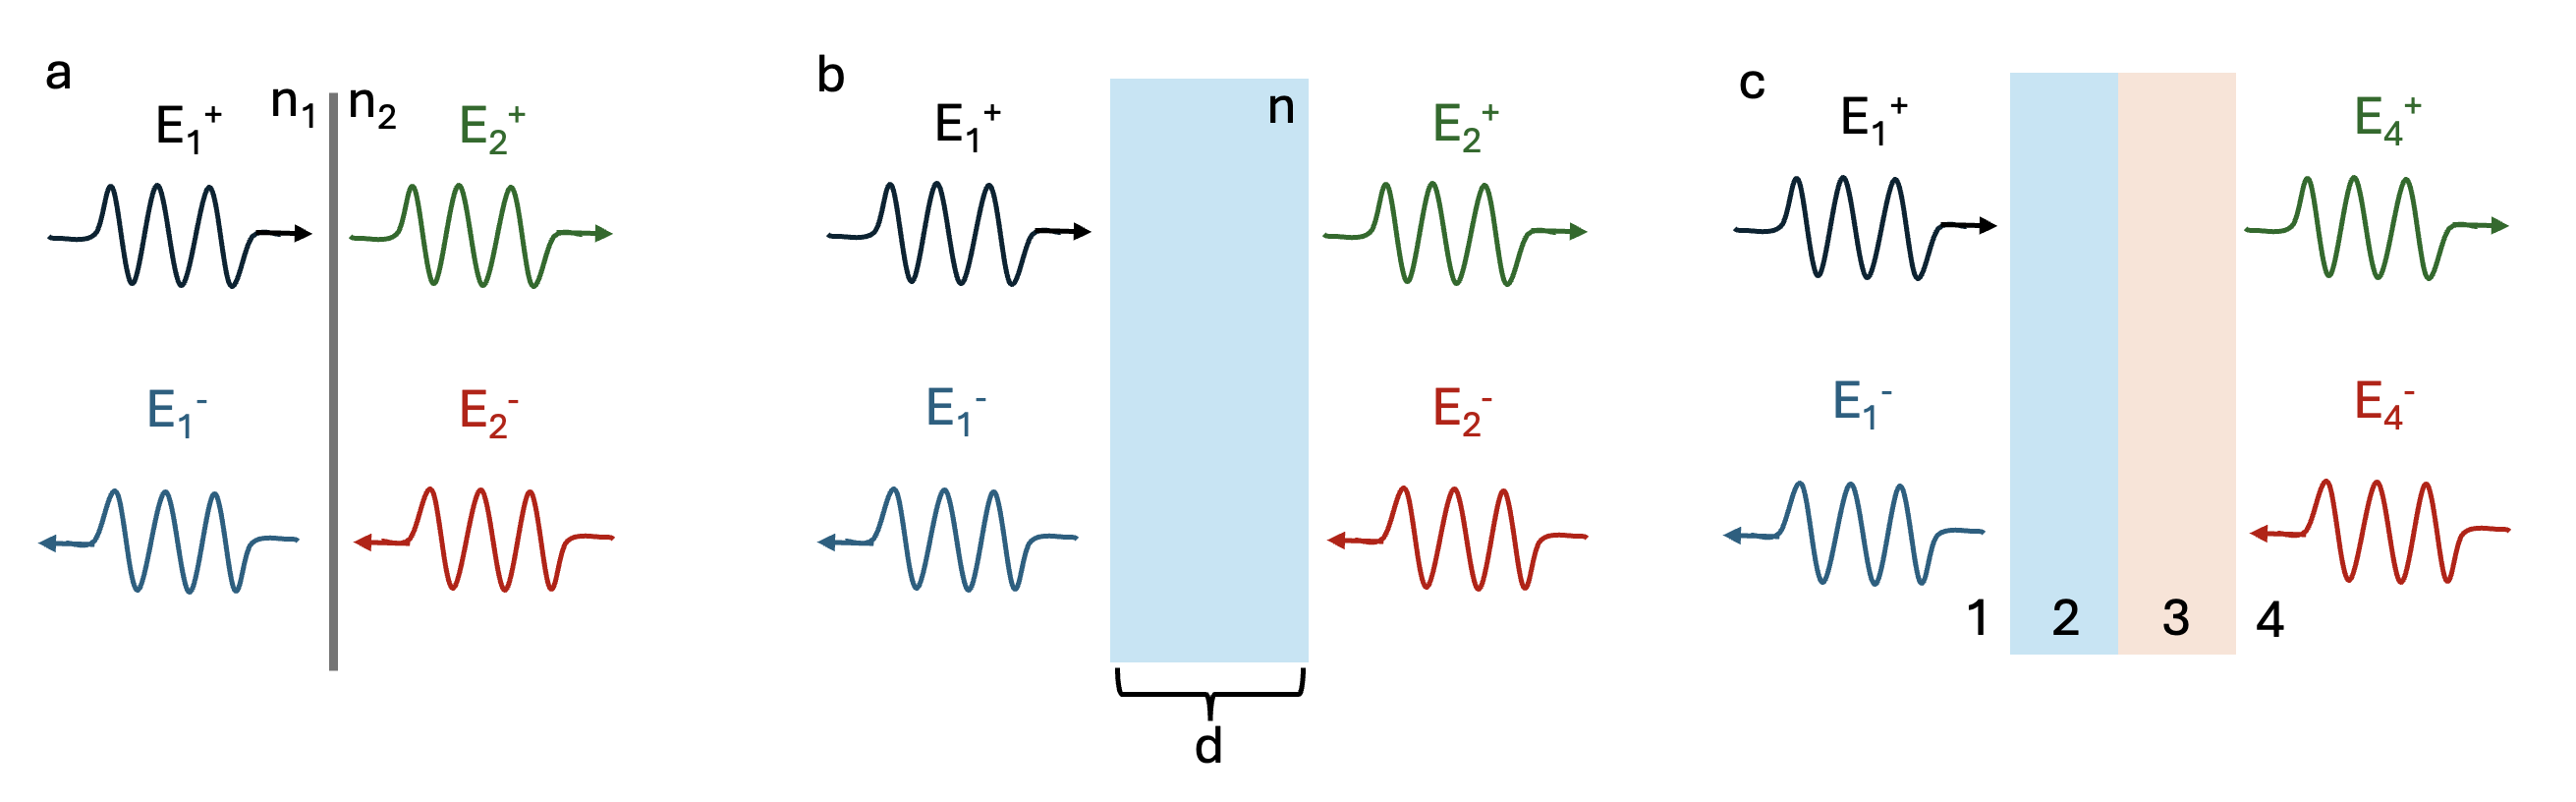
\includegraphics[width=1\textwidth]{figures/propagation.png}
	\caption[Propagation through different media]{Propagation of waves at an interface 
	(a), through a layer with refractive index $n$ and thickness $d$ (b), and through a multilayer system (c).}\label{fig: propagation}
\end{figure}
where $k = 2 \pi n / \lambda$ is the wavenumber in the medium. This analysis can be extended to a two layer system by multiplying the interface and propagation matrices while considering the order of the layers. Starting from the rightmost boundary as shown in~\ref{fig: propagation}c, the fields on both sides are related using the interface matrix by $\mathbf{E}_{3R} = \mathbf{D}_{34}\mathbf{E}_{4}$, where $3R$ is the field at the right side of layer $3$. The fields at the left side of layer $3$ are related to the right side by the propagation matrix $\mathbf{E}_{3L} = \mathbf{P}_3\mathbf{E}_{3R}$, which in turn can be related using another interface matrix to the field across the relevant boundary. This results in the following matrix equation relating the fields at the leftmost region to the rightmost region:

\begin{equation} \label{eqn: total_matrix}
	\mathbf{M}=\mathbf{D}_{12}\mathbf{P}_2\mathbf{D}_{23}\mathbf{P}_3\mathbf{D}_{34}
\end{equation}
such that 

\begin{equation} \label{eqn: transfer_matrix_fields}
	\begin{bmatrix} E_1^+ \\ E_1^- \end{bmatrix} = \mathbf{M} \begin{bmatrix} E_4^+ \\ E_4^- \end{bmatrix}= \begin{bmatrix}  M_{11} & M_{12} \\ M_{21} & M_{22} \end{bmatrix} \begin{bmatrix} E_4^+ \\ E_4^- \end{bmatrix}.
\end{equation}

This method allows the analysis of any multilayer system using matrix multiplication of the component interface $\mathbf{D}$ and propagation $\mathbf{P}$ matrices. The reflection coefficient $r$ for a multilayer structure is simply

\begin{equation} \label{eqn: multilayer_reflection_coefficient}
	r = \frac{M_{21}}{M_{11}}
\end{equation}
since $t = 1 / M_{11}$ and $r = M_{21} / M_{11}$.

\section{Electron beam physical vapor deposition of a-Si and SiO\texorpdfstring{$_{2}$}{2}}
Silicon and its native oxide SiO$_2$ are the most common materials used in the semiconductor industry. Thin films of Si and SiO$_2$ are used in microelectronics, photonics, and photovoltaic applications. These thin films are grown using methods ranging from physical vapor deposition, chemical vapor deposition, to thermal oxidation. Electron beam physical vapor deposition (EBPVD) or e-beam evaporation is one commonly utilized technique for depositing high-purity Si and SiO$_2$ films due to its high deposition rate, precise thickness control, and capability to vaporize high-melting-point materials.

SiO$_2$ is widely utilized due to its wide bandgap ($\approx 8.9\text{ eV}$), low refractive index ($n \approx 1.45 - 1.46$ in the visible spectrum), high chemical stability, and low dielectric loss for optical coatings (Macleod, 2010). While thermal oxidation can produce high-quality native SiO$_2$ from Si, it requires high temperatures ($>$\qty{300}{\celsius}) and is restricted to silicon substrates. Electron beam evaporation enables low-temperature deposition ($<$\qty{300}{\celsius}) on different substrates including polymers, glass, and compound semiconductors such as GaAs (Schiller et al., 1982). However, e-beam evaporating silica presents unique physical challenges—specifically dissociation during evaporation, sub-stoichiometry SiO$_2$, porosity, and intrinsic film stress (Ritter, 1972).

In e-beam evaporation, a high-energy electron beam ($6 - 10\text{ kV}$) is magnetically steered onto a high-purity target contained in a water-cooled copper crucible. The electron generation mechanism relies on Richardson-Dushman thermionic emission from a heated filament (typically tungsten):

\begin{equation} \label{eqn: thermionic_emission}
	J = A T^2 \exp\left( -\frac{\Phi}{k_B T} \right)
\end{equation}

where $J$ is the emission current density \unit{\ampere\per\square\meter}, $A \approx 1.2 \times 10^6$ \unit{\ampere\per\square\meter\square\kelvin} is the Richardson constant.$\Phi$ is the work function of the filament material \unit{\electronvolt}.$k_B$ is the Boltzmann constant and $T$ is the absolute temperature in \unit{\kelvin}. Emitted electrons are accelerated toward an anode using a high potential difference. The beam trajectory is controlled via the Lorentz force:

\begin{equation} \label{eqn: Lorentz}
		\textbf F=e(\textbf E+\textbf v \times\textbf B)
\end{equation}

In a uniform transverse magnetic field $\mathbf{B}$, electrons follow a circular path. This bending caused by the magnetic field allows the electron gun to remain shielded from direct line-of-sight deposition from the source while enabling frequent sweeping across the crucible to maintain uniform evaporation from the source as shown in~\ref{fig: polarization}. As the electron beam strikes the source, local temperatures at the beam spot may exceed $1700^\circ\text{C}$, causing melting and evaporation for Si or direct sublimation in the case of SiO$_2$ (Schiller et al., 1982). Unlike pure Si, SiO$_2$ does not evaporate purely as intact SiO$_2$ molecules. Thermal dissociation may occur at the surface of the source, yielding a mixture of gaseous species (Ritter, 1972):
\begin{equation} \label{eqn: sio_evap}
	\text{SiO}_2\,\text{(s)} \longrightarrow \text{SiO}\,\text{(g)} + \frac{1}{2}\text{O}_2\,\text{(g)}
\end{equation}
\begin{equation} \label{eqn: si_evap}
	\text{SiO}_2\,\text{(s)} \longrightarrow \text{Si}\,\text{(g)} + \text{O}_2\,\text{(g)}
\end{equation}

Unassisted e-beam evaporation of SiO$_2$ in high vacuum typically yields sub-stoichiometric films of SiO$_x$ where $x < 2.0$. Sub-stoichiometry impacts film performance by introducing sub-oxide states ($\text{Si}^{1+}$, $\text{Si}^{2+}$, $\text{Si}^{3+}$) and oxygen vacancies, leading to an increased optical absorption and increased refractive index. To ensure fully stoichiometric SiO$_2$, reactive e-beam evaporation can be performed by introducing oxygen gas into the chamber.

According to the structure zone model, the growth of the films proceed in three general steps (Thornton). The first step occurs when the vaporized molecules are transported towards the substrate, the second when they are adsorbed onto the surface of the substrate or growing film, their diffusion across the surface, and any chemical reactions that may involve their incorporation into the film or removal via thermal desorption or sputtering. The third step involves the movement of the molecules to their final locations via bulk diffusion and solid state reactions. 

Movchan and Demchishin classified film growth into distinct zones, with the morphology of the films depending strongly on the normalized homologous temperature $T_h = {T_{\text{sub}}}/{T_m}$ where $T_{\text{sub}}$ is the substrate temperature and $T_m$ is the melting point of the material in \unit{\kelvin}. At low temperatures ($T_h < 0.3$) surface diffusion is low,  and molecules essentially stick where they arrive, producing porous, tapered columnar structures. This is considered as Zone 1. At Zone 2 ($T_h < 0.5$) the temperatures are high enough to allow the surface diffusion fluxes to dominate over the arrival fluxes, but still low enough such that the bulk diffusion rates remain orders of magnitude less than the surface diffusion rates. When the temperature is high enough, bulk diffusion will dominate over all other processes and fully dense grains form. This is considered as Zone 3. The morphology of the films also has an effect on the refractive index, with porous films generally having a lower index compared to the bulk.

\section{Envelope method for refractive index}\label{sec: swanepoel}